\documentclass[11pt]{article}

\usepackage[margin=1in]{geometry}
\usepackage{amsmath}
\usepackage{amssymb}
\usepackage{booktabs}
\usepackage{graphicx}
\usepackage{xcolor}
\usepackage[font=small,labelfont=bf]{caption}
\usepackage{titlesec}
\usepackage{enumitem}
\usepackage[colorlinks=true,linkcolor=black,urlcolor=blue!60!black]{hyperref}

\definecolor{good}{HTML}{2E7D32}
\definecolor{bad}{HTML}{B3282D}
\definecolor{warn}{HTML}{B26A00}
\definecolor{box}{HTML}{F2F4F8}
\newcommand{\dg}{\ensuremath{^\circ}}
\newcommand{\dprime}{d'}
\newcommand{\dd}{\Delta d'}
\newcommand{\dc}{\Delta c}
\newcommand{\claimbox}[1]{\par\smallskip\noindent\colorbox{box}{\parbox{0.97\linewidth}{\vspace{1mm}#1\vspace{1mm}}}\par\smallskip}

\titleformat{\section}{\normalfont\large\bfseries}{\thesection}{0.6em}{}
\titleformat{\subsection}{\normalfont\normalsize\bfseries}{\thesubsection}{0.6em}{}

\title{\vspace{-1.3cm}\textbf{Attention as a signal-coherence mechanism}\\[2mm]
\large A synthesis of the VDA series, and what makes the cue effect large}
\author{Synthesis memo}
\date{18 August 2026}

\begin{document}
\maketitle
\vspace{-0.6cm}

\begin{abstract}
\noindent The VDA experiments have accumulated as a sequence of separately gated results:
psychometrics across set size, source-separated attention maps, a memory-noise pilot, a
spatial-discretization control, and a causal routing intervention. This memo argues they
form one story. The model's attention is not a sensory gain control. At the moment of the
change it puts $11\times$ \emph{less} than uniform weight on the changed location's
\emph{image} tokens while putting $2.1\times$ uniform weight on that location's
\emph{memory} state. What the cue buys is not a better look; it is a decision about which
stored trace to keep coherent and read out. Three further results follow that reading:
the memory-side allocation is graded by cue validity; boosting routing at the true change
location rescues a missed change ($\dd = +2.23$) while boosting the cued-but-wrong location
\emph{hurts} ($\dd = -1.78$) and a neutral control does nothing ($\dd = -0.30$); and the
sensitivity-corrected cueing effect grows $2.45\times$ from set size 4 to 16, exactly where
more competing traces must be held apart. A discretization control shows this is about
competing items, not finer grids: holding the task at four physical regions and raising
tokens from 4 to 100 does not increase the cueing cost. The registered test of the
coherence hypothesis --- the memory-noise pilot --- does \emph{not} support it: noise leaves
the cueing effect unchanged ($+0.404 \to +0.406$) and abolishes validity grading rather than
sharpening it. The coherence story therefore rests on allocation source, causal specificity,
and set-size scaling, not on interference. A closing section ranks the levers that make the
attention and cue effects most pronounced, and proposes a manuscript spine.
\end{abstract}

\section{The claim, stated so it can fail}

\claimbox{\textbf{Signal coherence.} In this model family, spatial attention operates on
\emph{stored} signal rather than incoming signal. Its function is to select which location's
recurrent memory trace the decision reads, and to protect that trace's integrity against
competition from the other locations. The cue's role is to nominate that location in advance.}

\noindent This is a stronger and more specific claim than ``the model attends to the cue.''
It makes four commitments, each of which the series can now test:

\begin{enumerate}[leftmargin=1.6em,itemsep=2pt]
\item \textbf{Source.} Selection should appear in the memory-side routing, not the image-side
routing. If attention were sensory gain, weight on the changed location's image tokens should
\emph{rise} at the change.
\item \textbf{Conditioning.} The allocation should be graded by how informative the cue is,
and should move from the cued location to the true location once the change is available.
\item \textbf{Causal sufficiency and specificity.} Forcing coherence at the true location
should recover a change the model otherwise misses; forcing it at a wrong location should not,
and should ideally hurt.
\item \textbf{Scaling.} The effect should grow with the number of competing traces, because
that is what makes keeping one coherent hard.
\end{enumerate}

Sections 2--5 take these in order. Section 6 asks whether the scaling result is really about
items. Section 7 answers the practical question of which manipulations make the effects
largest. Section 8 reports the one registered test that does not support the claim.

\section{Source: the selection is in memory, not in the image}

This is the load-bearing result and it is currently buried in a comparison file rather than
presented as a finding. In native VDA4 at a $18\dg$ change, with attention mass measured
against a uniform baseline of $0.25$ per location:

\begin{table}[h]
\centering\small
\caption{Source-separated attention mass, clean terminal VDA4 (iteration 19{,}999,
\texttt{crossattn1}, $d_\mathrm{mem}{=}128$), averaged over displayed validities
$0.25/0.5/0.75$. Uniform allocation is $0.25$.}
\label{tab:source}
\begin{tabular}{llrr}
\toprule
Period & Location & Image mass & Memory mass \\
\midrule
Cue (frames 1--4)    & cued location        & 0.153 & 0.282 \\
Change (frames 5--6) & true change location & \textbf{0.022} & \textbf{0.535} \\
\bottomrule
\end{tabular}
\end{table}

At the moment that matters, memory-side weight on the changed location is $2.1\times$
uniform while image-side weight is $0.022$ --- roughly $11\times$ \emph{below} uniform, and
$24\times$ below the memory-side value (Figure~\ref{fig:source}). The model is not looking
harder at the changed location. It is reading that location's stored state and actively
withdrawing image-side weight from it.

\begin{figure}[h]
\centering
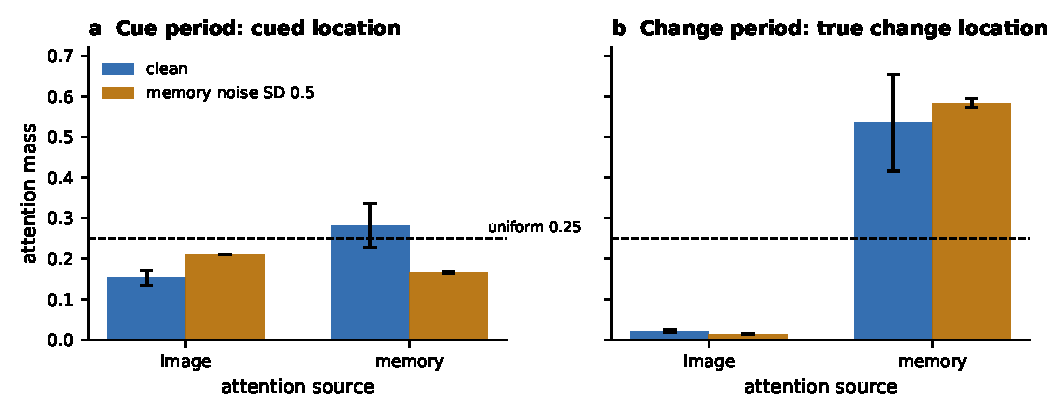
\includegraphics[width=\textwidth]{figs/fig2_source_dissociation.pdf}
\caption{Attention mass by source, VDA4. Bars are means over displayed validity; whiskers
span the validity range. Dashed line is uniform allocation. At the change, memory-side mass
on the true location is far above uniform while image-side mass is far below it. Adding
memory noise (orange) does not create this dissociation --- it is already the clean model's
strategy.}
\label{fig:source}
\end{figure}

\claimbox{\textbf{Why this matters for the paper.} A reader's default model of ``attention''
in a vision transformer is image-token weighting. The measured mechanism here is the
opposite. Every downstream result reads differently once this is established first, so it
should lead the results, not appear as a supplementary source-separation check.}

\section{Conditioning: the cue sets the coherence target, gradedly}

In the clean model, memory-side allocation scales with how informative the cue is
(Figure~\ref{fig:grading}). Cue-period mass on the cued location rises $0.234 \to 0.270 \to
0.341$ across displayed validity $0.25 \to 0.5 \to 0.75$ (slope $+0.108$), and change-period
mass on the true change location rises $0.432 \to 0.504 \to 0.670$ (slope $+0.238$). The
model is not applying a fixed spatial prior; it is scaling how much it commits to the cue
by how much the cue is worth.

\begin{figure}[h]
\centering
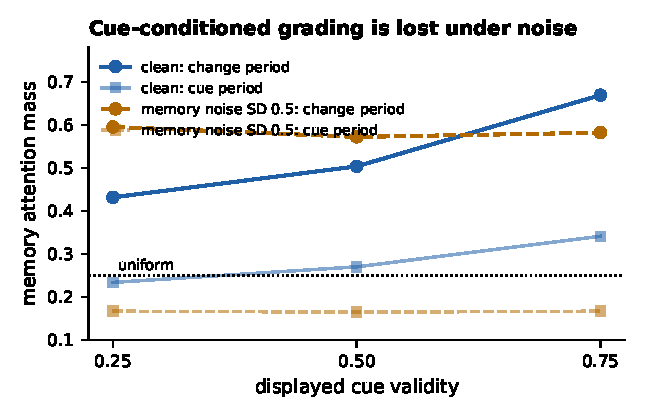
\includegraphics[width=0.55\textwidth]{figs/fig3_validity_grading.pdf}
\caption{Memory-side attention mass as a function of displayed cue validity. Clean model
(blue) grades its commitment with cue informativeness at both periods. The memory-noise
model (orange) is flat at both --- see Section~\ref{sec:noise}.}
\label{fig:grading}
\end{figure}

\section{Causal sufficiency and specificity: the rescue works, and only at the right place}

The manuscript marked this experiment pending. It is now complete. On VDA16 (affine,
terminal 19{,}999) with the cue at location 0, the change forced to location 15, and a
neutral control at location 5, routing keys were clamped from frame 5 over a dose ladder
$0 \to 1$:

\begin{table}[h]
\centering\small
\caption{Change-location intervention, VDA16 affine, forced-invalid stress test, 300 trials
per condition, common random numbers. Boost and suppress are the extreme doses.}
\label{tab:causal}
\begin{tabular}{lrrrr}
\toprule
Intervention site & Detection (suppress) & Detection (boost) & $\Delta$detection & $\dd$ \\
\midrule
True change location (15) & 0.747 & 0.993 & $+0.247$ & $\mathbf{+2.23}$ \\
Cued but wrong location (0) & 0.990 & 0.860 & $-0.130$ & $-1.78$ \\
Neutral control (5) & 0.980 & 0.947 & $-0.033$ & $-0.30$ \\
\bottomrule
\end{tabular}
\end{table}

\noindent Three things make this a strong result rather than a demonstration that clamping
logits changes behavior. First, the effect is \emph{signed by role}: coherence at the true
location helps, coherence at the cued-but-wrong location actively hurts, and the neutral
control is near zero. Second, the intervention verifiably moved what it was supposed to
move --- achieved mass at the true location went $0.445 \to 0.987$ across the dose range.
Third, the suppression arm establishes that the model's natural routing was already doing
the work: suppressing it drops detection from $0.98$ to $0.747$.

\begin{figure}[h]
\centering
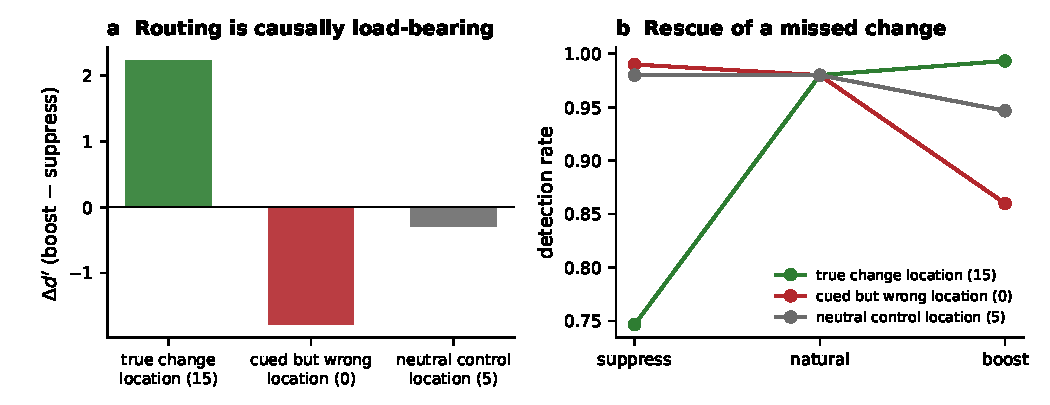
\includegraphics[width=\textwidth]{figs/fig4_causal_specificity.pdf}
\caption{Causal specificity. (a) Sensitivity change from suppressing to boosting routing at
three sites. (b) The same three sites across the dose ladder; only the true change location
shows rescue, and the cued-but-wrong site shows interference.}
\label{fig:causal}
\end{figure}

This is the model-level analogue of the Moore--Armstrong and Cavanaugh--Wurtz logic the
introduction invokes, and it is the series' single largest effect.

\section{Scaling: the effect grows with the number of competing traces}

Comparing terminal, architecture-matched checkpoints \emph{within the historical lineage}
(\texttt{crossattn1}, $d_\mathrm{mem}{=}128$, no decay, iteration 19{,}999), the
sensitivity-corrected cueing effect at $18\dg$ rises from $\dd = +0.404$ at set size 4 to
$\dd = +0.988$ at set size 16 --- a factor of $2.45$ (Figure~\ref{fig:setsize}). The
criterion shift roughly doubles as well ($-0.202 \to -0.494$), so the cue does move bias;
but the sensitivity component is real, grows, and is not an artifact of response rate.

\begin{figure}[h]
\centering
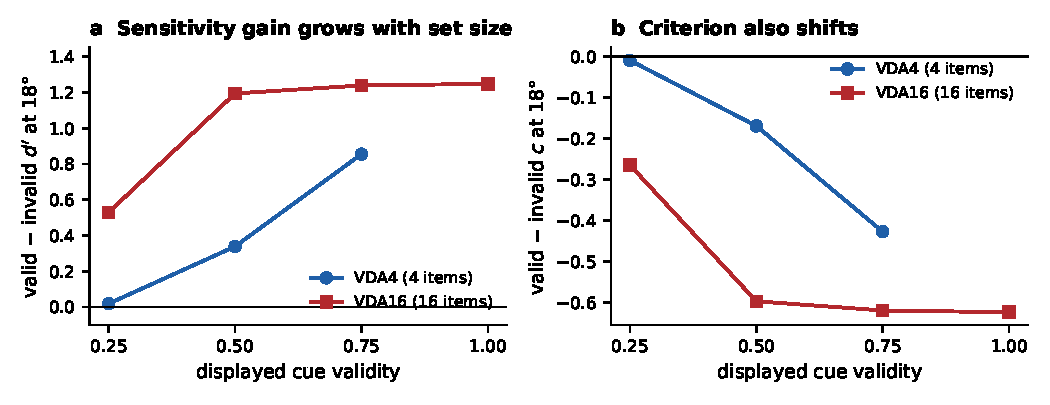
\includegraphics[width=\textwidth]{figs/fig1_setsize_sdt.pdf}
\caption{Cueing effect decomposed, at a $18\dg$ change. (a) Valid-minus-invalid $\dprime$
grows with set size at every validity. (b) The criterion shift grows too; the cue makes the
model both more sensitive and more willing at the cued location.}
\label{fig:setsize}
\end{figure}

Two details are worth keeping. Cue validity matters more at set size 4 in relative terms
--- the VDA4 effect nearly vanishes at validity $0.25$ ($\dd = +0.018$) and reaches
$+0.855$ at $0.75$ --- whereas VDA16 already shows $\dd = +0.529$ at validity $0.25$ and
saturates near $+1.25$. With four items the model can afford to ignore a weak cue; with
sixteen it cannot. That is what a coherence account predicts.

At set size 16 the two routing families are behaviorally near-identical
($\dd = +0.988$ cross-attention, $+0.946$ affine), which matters for Section~\ref{sec:disc}.

\section{Is it items or pixels? The discretization control}\label{sec:disc}

The set-size comparison confounds item count with grid geometry: VDA4 is $2\times2$ and
VDA16 is $4\times4$. The manuscript flags this as an open question. The spatial-scaling
experiment resolves it by holding the physical task at four regions and varying only the
token grid ($4$, $16$, $100$ tokens).

\begin{table}[h]
\centering\small
\caption{Spatial-scaling control at displayed validity 1.0, seed 0. The task has four
physical regions in every cell; only tokenization changes.}
\label{tab:disc}
\begin{tabular}{lrrrr}
\toprule
Routing family & Tokens & Threshold cost (deg) & Response AUC & Causal dependence (pp) \\
\midrule
Cross-attention & 4   & 7.16 & 0.219 & 12.4 \\
Cross-attention & 16  & 5.66 & 0.170 & 8.0 \\
Cross-attention & 100 & 6.18 & 0.197 & 1.2 \\
Affine EW       & 4   & 2.62 & 0.085 & 38.4 \\
Affine EW       & 16  & 2.60 & 0.079 & 98.0 \\
Affine EW       & 100 & 4.24 & 0.122 & 99.2 \\
\bottomrule
\end{tabular}
\end{table}

\noindent Finer discretization does not manufacture the set-size effect. Cross-attention's
threshold cost is non-monotonic and no larger at 100 tokens than at 4, and event-localized
attention concentration \emph{declines} ($0.748 \to 0.667 \to 0.355$). The $2.45\times$
growth from VDA4 to VDA16 is therefore attributable to competing items rather than to grid
resolution --- for this family and this seed (Figure~\ref{fig:disc}).

\begin{figure}[h]
\centering
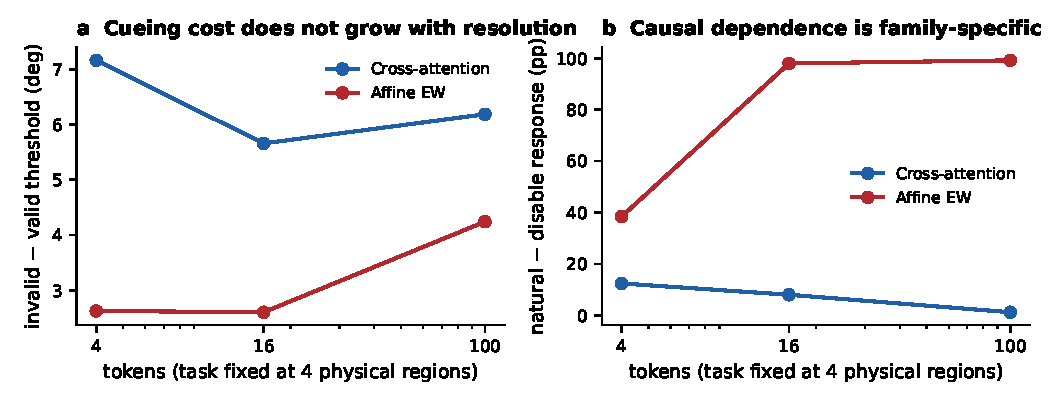
\includegraphics[width=\textwidth]{figs/fig5_discretization.pdf}
\caption{Discretization control. (a) Cueing cost does not grow with token count in either
family. (b) Causal dependence on routing diverges sharply: near-total for affine at high
token counts, near-zero for cross-attention.}
\label{fig:disc}
\end{figure}

The second panel carries an independent methodological point that deserves to be in the main
text. At set size 16 the two families produce nearly the same behavioral cueing effect
($+0.99$ vs $+0.95$), yet in the scaling control their dependence on routing differs by up to
$80\times$ ($1.2$ vs $99.2$ percentage points at 100 tokens). Cross-attention shows the
\emph{larger} behavioral cueing cost while depending on routing the \emph{least}.

\claimbox{\textbf{Behavior does not identify mechanism.} Two models can match on
psychometrics and cueing effects while differing almost totally in whether routing is
load-bearing. This is the strongest available argument for why the intervention experiments
are not optional garnish --- they are the only thing that distinguishes the families.}

\section{What makes the attention and cue effects most pronounced}

Ranked by measured effect on the cueing contrast (Figure~\ref{fig:levers}):

\begin{table}[h]
\centering\small
\caption{Levers, by how much they move the sensitivity-corrected cueing effect.}
\label{tab:levers}
\begin{tabular}{p{6.4cm}rp{6.2cm}}
\toprule
Lever & $\Delta$ in $\dprime$ units & Note \\
\midrule
Direct routing intervention at the true location & $+2.23$ & Largest effect in the series; requires a forced-invalid baseline to have headroom \\
Raising cue validity within VDA4 ($0.25 \to 0.75$) & $+0.84$ & Effect nearly vanishes at low validity \\
Raising cue validity within VDA16 ($0.25 \to 1.0$) & $+0.72$ & Saturates above validity $0.5$ \\
Set size $4 \to 16$ & $+0.58$ & The cleanest structural lever; $2.45\times$ multiplicative \\
Memory noise SD $0.5$ (VDA4) & $+0.00$ & No effect on the cueing contrast; see Section~\ref{sec:noise} \\
\bottomrule
\end{tabular}
\end{table}

\begin{figure}[h]
\centering
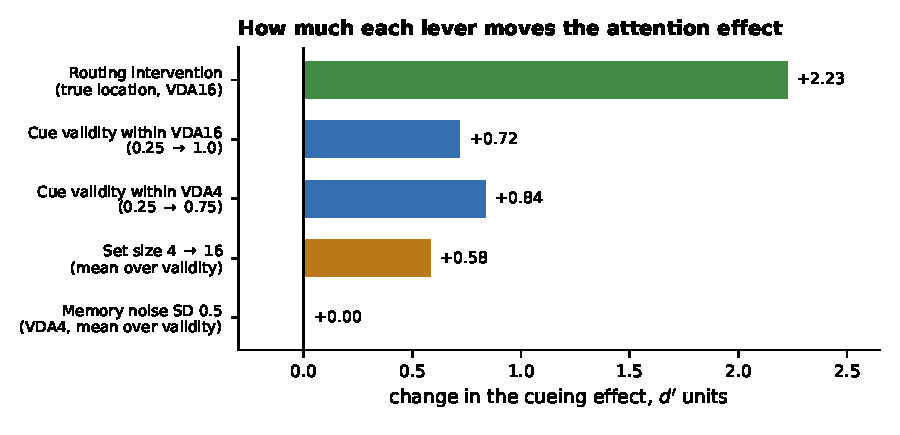
\includegraphics[width=0.86\textwidth]{figs/fig6_levers.pdf}
\caption{How much each manipulation moves the cueing effect, in $\dprime$ units.}
\label{fig:levers}
\end{figure}

Three practical points follow, and they are the design advice worth carrying into the next
round of experiments.

\textbf{Ceiling is the enemy.} At natural validity the VDA16 model detects a $30\dg$ change
on $98\%$ of trials. Nothing --- no cue manipulation, no intervention --- can show an effect
against that. The change-location experiment only produced a $+2.23$ effect because the
forced-invalid stress test plus routing suppression pushed the baseline down to $0.747$.
\emph{Manufacture headroom first, then manipulate.}

\textbf{Use the validity ladder, not a single validity.} At VDA4 the cueing effect ranges
from $+0.018$ to $+0.855$ across displayed validity. A single-validity design would have
reported either a null or a large effect depending on an arbitrary choice.

\textbf{Combine set size with forced-invalid probes.} These are the two structural levers
that operate without touching the model. Set size 16 with forced-invalid trials at moderate
change magnitude is the regime where the attention effect, the allocation signature, and the
causal intervention are all simultaneously measurable.

\section{The registered test that does not support the claim}\label{sec:noise}

The memory-noise pilot was designed as \emph{the} test of the signal-coherence hypothesis.
Its own pre-registered interpretation plan requires three things to align: a
sensitivity-corrected cueing effect that \emph{increases} under noise, allocation that
becomes \emph{more} selectively cue- and target-aligned, and spatially specific causal
dependence. Measured against that standard, the arm does not support the hypothesis.

\begin{table}[h]
\centering\small
\caption{Memory-noise pilot against its own registered requirements. Clean model is terminal
(19{,}999); the noisy model is an interrupted checkpoint (15{,}999), and both training-time
and evaluation-time noise change together.}
\label{tab:noise}
\begin{tabular}{p{5.4cm}p{2.6cm}p{6.4cm}}
\toprule
Requirement & Outcome & Measured \\
\midrule
Cueing effect increases under noise & \textcolor{bad}{not met} & $\dd = +0.404 \to +0.406$; difference $+0.002$ \\
Allocation becomes more cue-aligned & \textcolor{bad}{not met} & Cue-period cued memory mass \emph{falls} $0.282 \to 0.166$, below uniform \\
Allocation becomes more target-aligned & \textcolor{warn}{partial} & Change-period target memory mass $0.535 \to 0.584$, but validity grading is abolished (slope $+0.238 \to -0.013$) \\
Spatially specific causal dependence & not tested & No intervention was run in this arm \\
\bottomrule
\end{tabular}
\end{table}

\noindent By the pilot's own interpretation table this is ``descriptive redistribution only;
no signal-coherence support.'' The result is also confounded: the noisy model stopped at
$80\%$ of training, and the contrast changes training-time and evaluation-time noise
simultaneously, so it cannot separate learned compensation from acute corruption.

There is still something to report, but it is a different finding from the one that was
sought. Under memory noise the model \emph{stops using the cue} --- allocation goes flat
across validity at both periods --- and falls back on a uniform, stimulus-driven
concentration on the target after the change. That is a substitution of strategy, not an
intensification of one. It is interesting, and it should be written up as such rather than
as weak evidence for coherence.

\claimbox{\textbf{Recommendation.} Do not hang the coherence thesis on interference. The
thesis is carried by Sections 2--5: allocation source, cue-conditioned grading, causal
specificity, and set-size scaling. Re-run the noise arm properly paired (matched iteration,
factorial train-noise $\times$ eval-noise, with the intervention included) and let it be its
own question.}

\section{What the synthesis still needs}

\begin{itemize}[leftmargin=1.4em,itemsep=2pt]
\item \textbf{Seeds.} Every quantitative claim above is seed 0. The spatial-scaling
experiment has one seed-1 replication cell; nothing else does. Any statement of the form
``the effect grows $2.45\times$'' is a within-checkpoint measurement, not a population estimate.
\item \textbf{The intervention exists at one set size and one family.} The causal result is
VDA16 affine. The set-size scaling result is cross-attention. The cleanest missing experiment
is the change-location intervention run at VDA4 \emph{and} VDA16 in \emph{both} families ---
that single $2\times2$ would let the causal effect inherit the set-size claim instead of
sitting beside it.
\item \textbf{Source separation at VDA16.} The image-versus-memory dissociation is measured
at VDA4. If it holds at VDA16 the coherence story becomes considerably stronger, because
that is where competition is greatest.
\item \textbf{Lineage discipline.} The set-size comparison here sits within the historical
lineage. The manuscript's controlled-lineage numbers tell the same story in response-rate
terms: a valid-minus-invalid gap of $0.52$ at set size 16, and valid versus invalid
thresholds of $12.0\dg$ and $17.3\dg$ at set size 4, against $16.0\dg$ and $26.9\dg$ at set
size 16. Both should be reported; they must not be pooled.
\end{itemize}

\section{Proposed manuscript spine}

The current manuscript is ordered behavior $\rightarrow$ attention $\rightarrow$ intervention,
following the reference paper. That order buries the most distinctive finding. A coherence-led
spine:

\begin{enumerate}[leftmargin=1.6em,itemsep=2pt]
\item \textbf{Attention here is not sensory gain} (Section 2). Source-separated allocation,
VDA4, with the $0.022$ versus $0.535$ contrast as the paper's first figure.
\item \textbf{The cue nominates a trace, gradedly} (Section 3). Validity grading of
memory-side mass.
\item \textbf{The nomination is causally load-bearing} (Section 4). The rescue, with its
signed specificity across three sites.
\item \textbf{Coherence matters more with more competitors} (Section 5), with the
discretization control (Section 6) immediately after, so the confound is closed in place
rather than deferred to a discussion caveat.
\item \textbf{Behavior does not identify mechanism} (Section~\ref{sec:disc}) as the
methodological pivot that justifies the intervention program.
\item \textbf{Interference is a separate, open question} (Section~\ref{sec:noise}), reported
honestly as a strategy substitution with a null on the registered primary.
\end{enumerate}

\noindent The existing evidence-class apparatus, provenance appendices, and the historical
versus controlled lineage discipline carry over unchanged; this is a reordering of the
argument, not a relaxation of its gates.

\end{document}
